\newpage
\section{Questão 12-47}

\begin{figure}[H]
	\centering
	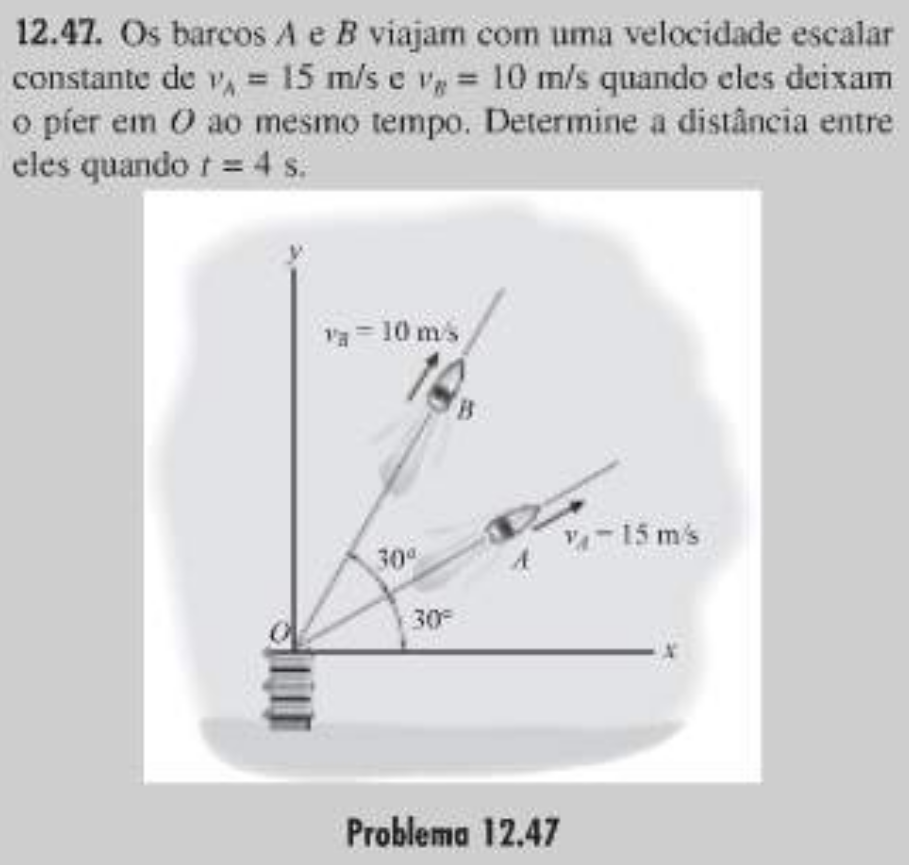
\includegraphics[width=.7\linewidth]{fundamentais/12-47.png}
	\caption{Comando da questão 12-47.}\label{fig:12-47}
\end{figure}

Nesta questão, analisamos o movimento de dois barcos, \(A\) e \(B\), que se movem em direções diferentes. O barco \(A\) se move com uma velocidade escalar \(v_A = 15 \, \text{m/s}\) a um ângulo de \(30^\circ\) em relação ao eixo \(x\), enquanto o barco \(B\) se move com uma velocidade escalar \(v_B = 10 \, \text{m/s}\) na direção do eixo \(y\). Determinamos a distância entre os barcos no instante \(t = 4 \, \text{s}\).

\subsection*{Movmento relativo:}
A velocidade do barco \(A\) é dada por suas componentes \(v_A\) e \(v_{B/A}\):

\[
v_B = v_A + v_{B/A}
\]
\[
x_A = v_A \cdot t \cdot \cos(\theta),
\]
\[
y_A = v_A \cdot t \cdot \sin(\theta),
\]
onde:
\begin{itemize}
    \item \(v_A = 15 \, \text{m/s}\) é a velocidade escalar do barco \(A\);
    \item \(\theta = 30^\circ = \frac{\pi}{6}\) é o ângulo do movimento do barco \(A\).
\end{itemize}

A posição do barco \(B\) é:
\[
x_B = 0, \quad y_B = v_B \cdot t,
\]
onde \(v_B = 10 \, \text{m/s}\) é a velocidade escalar do barco \(B\).

\subsection*{Distância entre os Barcos}
A distância entre os barcos é dada por:
\[
d(t) = \sqrt{(x_A - x_B)^2 + (y_A - y_B)^2}.
\]

Substituímos as expressões para \(x_A\), \(x_B\), \(y_A\) e \(y_B\):
\[
d(t) = \sqrt{\left(v_A \cdot t \cdot \cos(\theta) - 0\right)^2 + \left(v_A \cdot t \cdot \sin(\theta) - v_B \cdot t\right)^2}.
\]

Simplificando:
\[
d(t) = \sqrt{\left(15 \cdot t \cdot \cos\left(\frac{\pi}{6}\right)\right)^2 + \left(15 \cdot t \cdot \sin\left(\frac{\pi}{6}\right) - 10 \cdot t\right)^2}.
\]

\subsection*{Cálculo para \(t = 4 \, \text{s}\)}
Substituímos \(t = 4 \, \text{s}\) na expressão:
\[
d(4) = \sqrt{\left(15 \cdot 4 \cdot \cos\left(\frac{\pi}{6}\right)\right)^2 + \left(15 \cdot 4 \cdot \sin\left(\frac{\pi}{6}\right) - 10 \cdot 4\right)^2}.
\]

Calculando:
\[
\cos\left(\frac{\pi}{6}\right) = \frac{\sqrt{3}}{2}, \quad \sin\left(\frac{\pi}{6}\right) = \frac{1}{2}.
\]

Substituímos:
\[
d(4) = \sqrt{\left(15 \cdot 4 \cdot \frac{\sqrt{3}}{2}\right)^2 + \left(15 \cdot 4 \cdot \frac{1}{2} - 10 \cdot 4\right)^2}.
\]

Simplificando:
\[
d(4) = \sqrt{\left(60 \cdot \frac{\sqrt{3}}{2}\right)^2 + \left(30 - 40\right)^2},
\]
\[
d(4) = \sqrt{\left(30\sqrt{3}\right)^2 + (-10)^2}.
\]

Calculando:
\[
d(4) = \sqrt{2700 + 100} = \sqrt{2800} \approx 52.92 \, \text{m}.
\]

\subsection*{Resultado Final}
A distância entre os barcos no instante \(t = 4 \, \text{s}\) é:
\[
d(4) \approx 52.92 \, \text{m}.
\]
